\documentclass{../Common/Structure/doc_pdf}

\titleSubtitle{{\Huge\textit{Power EnJoy}}\\{\LARGE Integration Test Plan Document}}{Version 1.0.0}
\pageHeader{Integration Test Plan Document}

\begin{document}
\titleToc

\chapter{Introduction}
This document represent the Requirement Analysis and Specification Document (RASD). The main goal of this document is to completely describe the system in terms of functional and non-functional requirements, analyse the real need of the customer to modelling the system, show the constraints and the limit of the software and simulate the typical use cases that will occur after the development. This document is intended to all developer and programmer who have to implement the requirements, to system analyst who want to integrate other system with this one, and could be used as a contractual basis between the customer and the developer.
\section{List of definitions and abbreviations}
\paragraph{Definitions}
In the document are often used some specific terms whose definitions are reported bellow:
\begin{itemize}
	\item Server Database: data layer
	\item Server Application: application layer
	\item Client: client layer
	\item Mobile App: \textit{myTaxiService} mobile application, in Client
	\item Web App: \textit{myTaxiService} web application, in Client
	\item System: the union of software and hardware to be developed and implemented
	\itemBold{Integration Test Case} An atomic procedure done to test the integration of a component on the top of another one.
	\itemBold{Integration Test Suite} A collection of \textbf{Integration Test Cases}.
	\item See the correspondent section in the \textbf{RASD} and the \textbf{DD} for more definitions.
\end{itemize}
\paragraph{Acronyms}
\begin{itemize}
	\itemBold{RASD Requirements Analysis and Specification Document
	\itemBold{DD} Design Document
	\itemBold{API} Application Programming Interface
	\itemBold{DBMS} DataBase Management System
	\itemBold{ITPD} Integration Test Plan Document.
	\itemBold{In} Integration Test Suite number n.
	\itemBold{InTm} Integration Test Case number m of the Integration Test Suite number n.
	\itemBold{JS} JavaScript.
	\itemBold{UI} User Interface.
	\item See the correspondent section in the \textbf{RASD} and the \textbf{DD} for more acronyms and abbreviations.
\end{itemize}

\section{List of reference documents}
\begin{itemize}
	\item Software Engineering 2 Project AA 2016/2017: Project Description And Rules and Assignment 4 - integration test plan
	\item PowerEnJoy's Requirement Analysis and Specification Document (RASD)
	\item PowerEnJoy's Design Document (DD)
\end{itemize}
\newpage

\chapter{Integration Strategy}
\section{Entry Criteria}
Before starting the integration testing of any software component that has been designed for \PowerEnJoy{} system, the internal functions of the considered component (i.e. public or protected methods that are exposed within the package of the component but are not part of any external public interface) must be unit tested using an appropriate framework.
\section{Elements to be integrated}
\PowerEnJoy{} as shown in the \textbf{DD} is a three-tier system composed by:
\begin{itemize}
	\itemBold{DBMS} The memory of \PowerEnJoy{} entire system
	\itemBold{PowerEnJoy System} The main server and the main core composed by:
		\begin{enumerate}
			\item Data Manager
			\item Account Manager
			\item Ride Manager
			\item Bill Manager
			\item Map Services
			\item Notification
			\item Car Manager
			\item Zone Manager
			\item Problem Manager
		\end{enumerate}
	\itemBold{Client Application} Subdivided in \textbf{Car System} and \textbf{Mobile Application}
\end{itemize}
Moreover we assume that that Google Maps API and Paypal are well tested by their owner and thus we can use them without testing any further.

\section{Integration testing strategy}
The integration testing strategy, conducted in this project, is a \textbf{bottom-up} approach. This strategy tests the lower level components and start testing a way upwards to higher level components. The advantage of this strategy is that allow us to maintain the code easier, smaller modules have unit tests and there is a clearer structure of how to do things. The disadvantage is that when releasing a prototype it's impossible to see a working prototype until nearly all the program has been completed so that may take a long time before this happens. In early development, testing tools as Mockito and Arquillian (described in Chapter 4) allow us to test components which depend on incomplete ones through stubs and drivers (Chapter 5). The usage of the selected approach will create a robust application with efforts concentrated in testing the Server parts before all. 
%probably the component view needs to be changed in DD
\section{Sequence of component/function integration}
\subsection{Software integration sequence}
The following diagram illustrates the integration sequence of the various components, following the integration testing strategy described above. This means that in each subsystem, components are integrated starting from the most independent to the less independent, in order to prompt the chosen approach and improving modularity. 
\begin{center}
	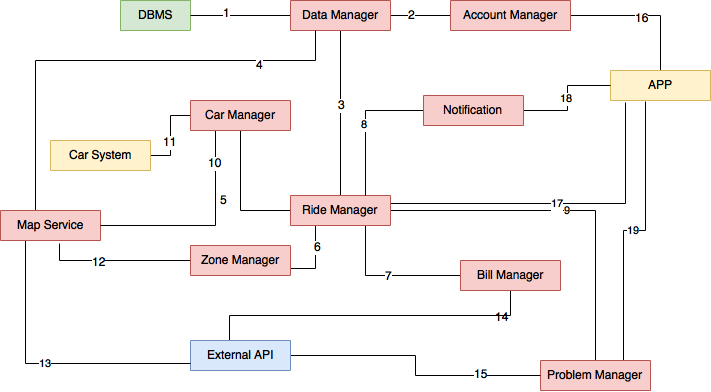
\includegraphics[width=\textwidth]{Diagrams/SoftwareIntegrationDiagram.png}
	\captionof{figure}{Software Integration Diagram}
	\label{Software Integration Diagram}
\end{center}

\subsection{Subsystem integration sequence}
The following diagram illustrates the integration sequence of the various subsystems, following the integration testing strategy described above. In particular, the Server Database is integrated before the Client, because the former does not need an actual functioning system in order to be tested efficiently, contrary to the latter.
%Image
\begin{center}
	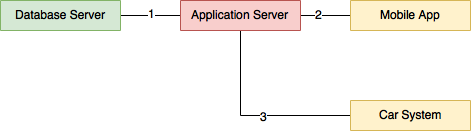
\includegraphics[width=\textwidth]{Diagrams/SubsystemsIntegrationDiagram.png}
	\captionof{figure}{Subsystem Integration Diagram}
	\label{Subsystem Integration Diagram}
\end{center}


\section{Component View}
\showRotateImage{Resources/ComponentDiagram.png}{Component diagram of the entire system}{1.4}{fig:Component}{0em}
\section{Deployment view}
\showPercentImage{Resources/DeploymentDiagram.png}{deployment diagram for PowerEnJoy}{1}{fig:Deploy}{0.5em}
\section{Runtime view}

	\showPercentImage{Resources/LoginSequence.png}{Login Sequence}{1}{fig:LogSeq}{0.5em}
	\newpage
	\showPercentImage{Resources/RegistrationSequence.png}{Registration Sequence}{1}{fig:RegSeq}{0.5em}

	\showPercentImage{Resources/FindFreeCarSequence.png}{Free Car sequence}{1}{fig:FreeSeq}{0.5em}

	\showPercentImage{Resources/ReserveSequence.png}{Reservation Sequence}{1}{fig:RevSeq}{0.5em}

	\showPercentImage{Resources/RentSequence.png}{Rent Sequence}{1}{fig:RentSeq}{0.5em}

	\showPercentImage{Resources/EndRentSequence.png}{End rent sequence}{1}{fig:EndRentSeq}{0.5em}

\newpage

\section{Component interfaces}
This section describes all interfaces between components, their interaction and their input/output parameters. For further, detailed explanations about their functioning, dependencies, resources, operations and parameters read the RASD release.

\subsection{Application$\leftrightarrow$Client Interface}
	\begin{itemize}
		\item [] \textbf{Components}:
			\begin{itemize}
				\item PowerEnJoyServer  (Application)
				\item Mobile App (Client)
			\end{itemize}			
		\item [] \textbf{Communication system}: JPA, JDBC APIs;
		\item [] \textbf{Protocols}: standard HTTPS protocol;
	\end{itemize}
	
\subsection{Application$\leftrightarrow$Database  Interface}
	\begin{itemize}
		\item [] \textbf{Components}:
		\begin{itemize}
			\item Data Manager (PowerEnJoyServer) (Application)
			\item PowerEnjoy DB (Database)
		\end{itemize}			
		\item [] \textbf{Communication system}: JPA, JDBC APIs;
		\item [] \textbf{Protocols}: standard TCP/IP protocols;
	\end{itemize}
	
\subsection{Map services}
	\begin{center}
		\begin{tabular}{ l | c | l   r }
			\multirow{2}{*}{\textbf{Operation}} & \textbf{Involved} & \textbf{Input/Output} & \multirow{2}{*}{[type]}\\
			& \textbf{Users} & \textbf{Parameters} & \\ [1.5ex]
			\hline\hline\\
			
			% GENERAL
			\multirow{2}{*}{\textit{(General)}}
				& \multirow{2}{*}{\textit{(All)}}
					&	token & [/]\\
					&&	errors & [/]\\ [1.5ex]
			\hline\\
			
			% Zone Management
			\multirow{2}{*}{\textbf{Zones Management}}
				& \multirow{2}{*}{Drivers}
					&	location & [Position]\\
					&&	available car & [Car]\\ [1.5ex]
			\hline\\
			
			% Google API
			\multirow{2}{*}{\textbf{Google Maps APIs}}
				& \multirow{1}{*}{Drivers}
					&	address & [string]\\
					&&	location car & [Position]\\ [1.5ex]
			\hline\\
			
		\end{tabular}
	\end{center}
	
\subsection{Account manager}
	\begin{center}
		\begin{tabular}{ l | c | l   r }
			\multirow{2}{*}{\textbf{Operation}} & \textbf{Involved} & \textbf{Input/Output} & \multirow{2}{*}{[type]}\\
			& \textbf{Users} & \textbf{Parameters} & \\ [1.5ex]
			\hline\hline\\
			
			% GENERAL
			\multirow{2}{*}{\textit{(General)}}
				& \multirow{2}{*}{\textit{(All)}}
					&	token & [/]\\
					&&	errors & [/]\\ [1.5ex]
			\hline\\
			
			% REGISTRATION
			\multirow{4}{*}{\textbf{Registration}}
			\multirow{4}{*}
				& \multirow{4}{*}{Visitors}
					&	email & [string]\\
					&&	password & [string]\\
					&& 	license ID & [string]\\
					&&	.. .& \\ [1.5ex]
			\hline\\
			
			% LOGIN
			\multirow{2}{*}{\textbf{Login}}
				& \multirow{2}{*}{Visitors}
					&	email & [string]\\
					&&	password & [string]\\ [1.5ex]
			\hline\\
			
			% EMAIL CONFIRMATION
			\multirow{2}{*}{\textbf{Email Confirmation}}
				& \multirow{1}{*}{Driver}
					&	\multirow{2}{*}{password} & \multirow{2}{*}{[string]}\\ [1.5ex]
			\hline\\
			
			% PROFILE EDITING
			\multirow{4}{*}{\textbf{Profile Editing}}
				& \multirow{2}{*}{Drivers}
					& new email & [string]\\
					&& ... & \\ [1.5ex]
			\hline\\
			
			% PROFILE DELETING
			\multirow{2}{*}{\textbf{Profile Deleting}}
				& \multirow{2}{*}{Drivers}
					&	token & [/]\\
					&&	password & [string]\\ [1.5ex]
			\hline
		\end{tabular}
	\end{center}

	
\subsection{Notification}
	\begin{center}
		\begin{tabular}{ l | c | l   r }
			\multirow{2}{*}{\textbf{Operation}} & \textbf{Involved} & \textbf{Input/Output} & \multirow{2}{*}{[type]}\\
			& \textbf{Users} & \textbf{Parameters} & \\ [1.5ex]
			\hline\hline\\
			
			% GENERAL
			\multirow{2}{*}{\textit{(General)}}
				& \multirow{2}{*}{\textit{(All)}}
					&	token & [/]\\
					&&	errors & [/]\\ [1.5ex]
			\hline\\
			
			% Car Reservation NOTIFICATION
			\multirow{4}{*}{\textbf{Car Reservation Notification}}
				& \multirow{4}{*}{Drivers}
					&	car location & [Position]\\
					&&	ETA & [interval]\\
					&&	car state & [boolean]\\
					&&	... & \\ [1.5ex]
			\hline\\
			
			% BILL RIDE NOTIFICATION
			\multirow{4}{*}{\textbf{Bill Ride Notification}}
				& \multirow{4}{*}{Drivers}
					&	time of rent & [Time]\\
					&&	total amount & [float]\\
					&&	discount & [float]\\
					&&	... & \\ [1.5ex]
			\hline
		\end{tabular}
	\end{center}


\subsection{Ride manager}
	\begin{center}
		\begin{tabular}{ l | c | l   r }
			\multirow{2}{*}{\textbf{Operation}} & \textbf{Involved} & \textbf{Input/Output} & \multirow{2}{*}{[type]}\\
			& \textbf{Users} & \textbf{Parameters} & \\ [1.5ex]
			\hline\hline\\
			
			% GENERAL
			\multirow{2}{*}{\textit{(General)}}
				& \multirow{2}{*}{\textit{(All)}}
					&	token & [/]\\
					&&	errors & [/]\\ [1.5ex]
			\hline\\
			
			% RIDE REQUEST
			\multirow{9}{*}{\textbf{Ride Management}}
				& \multirow{9}{*}{Drivers}
					&	user ID & [string]\\
					&&	start location & [Position]\\
					&&	start time & [Time]\\
					&&	end time & [Time]\\
					&&	end location & [Position]\\
					&&	num passengers & [int]\\
					&&	battery state & [float]\\
					&&	bill & [float]\\
					&&	... & \\ [1.5ex]
			\hline\\
			
			% Reservation
			\multirow{2}{*}{\textbf{Reservation Update}}
				& \multirow{2}{*}{Drivers}
					&	request status & [enum]\\
					&&	new request status & [enum]\\ [1.5ex]
			\hline\\
			
			% Ride update
			\multirow{2}{*}{\textbf{Request Status Update}}
				& \multirow{2}{*}{Drivers}
					&	ride status & [enum]\\
					&&	new ride status & [enum]\\ [1.5ex]
			\hline\\

		\end{tabular}
	\end{center}

\subsection{Zone manager}
	\begin{center}
		\begin{tabular}{ l | c | l   r }
			\multirow{2}{*}{\textbf{Operation}} & \textbf{Involved} & \textbf{Input/Output} & \multirow{2}{*}{[type]}\\
			& \textbf{Users} & \textbf{Parameters} & \\ [1.5ex]
			\hline\hline\\
			
			% GENERAL
			\multirow{2}{*}{\textit{(General)}}
				& \multirow{2}{*}{\textit{(All)}}
					&	token & [/]\\
					&&	errors & [/]\\ [1.5ex]
			\hline\\
			
			\multirow{9}{*}{\textbf{Zone Management}}
				& \multirow{9}{*}{Drivers}
					&	car location & [Position]\\
					&&	discount & [float]\\
					&&	car state & [boolean]\\
					&&	... & \\ [1.5ex]
			\hline\\
			
			\multirow{2}{*}{\textbf{Zone Update}}
				& \multirow{2}{*}{Drivers}
					&	status & [enum]\\
					&&	new zone  & [Zone]\\ [1.5ex]
			\hline\\

		\end{tabular}
	\end{center}

\subsection{Bill manager}
	\begin{center}
		\begin{tabular}{ l | c | l   r }
			\multirow{2}{*}{\textbf{Operation}} & \textbf{Involved} & \textbf{Input/Output} & \multirow{2}{*}{[type]}\\
			& \textbf{Users} & \textbf{Parameters} & \\ [1.5ex]
			\hline\hline\\
			
			% GENERAL
			\multirow{2}{*}{\textit{(General)}}
				& \multirow{2}{*}{\textit{(All)}}
					&	token & [/]\\
					&&	errors & [/]\\ [1.5ex]
			\hline\\
			
			\multirow{9}{*}{\textbf{Bill Management}}
				& \multirow{9}{*}{Drivers}
					&	car location & [Position]\\
					&&	battery state & [float]\\
					&&	num passengers & [int]\\
					&&	time charged & [float]\\
					&&	... & \\ [1.5ex]
			\hline\\
			
			\multirow{2}{*}{\textbf{PayPal APIs}}
				& \multirow{2}{*}{Drivers}
					&	email & [string]\\
					&&	total amount & [float]\\ [1.5ex]
			\hline\\

		\end{tabular}
	\end{center}

\subsection{Car manager}
	\begin{center}
		\begin{tabular}{ l | c | l   r }
			\multirow{2}{*}{\textbf{Operation}} & \textbf{Involved} & \textbf{Input/Output} & \multirow{2}{*}{[type]}\\
			& \textbf{Users} & \textbf{Parameters} & \\ [1.5ex]
			\hline\hline\\
			
			% GENERAL
			\multirow{2}{*}{\textit{(General)}}
				& \multirow{2}{*}{\textit{(All)}}
					&	token & [/]\\
					&&	errors & [/]\\ [1.5ex]
			\hline\\
			
			% RIDE REQUEST
			\multirow{9}{*}{\textbf{Car Management}}
				& \multirow{9}{*}{Drivers}
					&	car location & [Position]\\
					&&	battery state & [float]\\
					&&	num passengers & [int]\\
					&&	time charged & [float]\\
					&&	... & \\ [1.5ex]
			\hline\\
			
			\multirow{2}{*}{\textbf{Car Update}}
				& \multirow{2}{*}{Drivers}
					&	new car status & [enum]\\
					&&	new car location & [Position]\\ [1.5ex]
			\hline\\

		\end{tabular}
	\end{center}
	
\subsection{Application$\leftrightarrow$Problem Manager Interface}
	\begin{itemize}
		\item [] \textbf{Components}:
			\begin{itemize}
				\item Problem Manager APIs
				\item Mobile App (Client)
			\end{itemize}			
		\item [] \textbf{Communication system}: JAX-RS API (RESTful interface)
		\item [] \textbf{Protocols}: standard HTTPS protocol;
	\end{itemize}

\subsection{Data manager}
	See subsection 2.6.1, \textit{"Application$\leftrightarrow$Database Interface"}.
\section{Selected architectural styles and patterns}
Various architectural and logical choices have been justified as following:

\begin{itemize}

	\item A \textbf{3-tier architecture} has been used: client, server application and server database.\\
	This is due to the fact that we're developing an overall light application that doesn't need a lot of computing power, especially on the client side. Therefore, it is possible to structure the system in a logically simple and easily understandable way, without having to lose much in terms of optimization. Besides, this allows to obtain a good compromise between thin client and database tiers, and a clear correspondence between tiers and layers (i.e. no layer is distributed among multiple tiers).

	\item For similar reasons, a \textbf{SOA (Service Oriented Architecture)} has been chosen for the communication of the application server with the front ends. This improves flexibility, through modularity and a clear documentation, and simplicity, through an higher abstraction of the components.

	\item The entire system is designed within the principles of \textbf{Modular programming}, focusing on assigning each functionality to a different module. This greatly improves extensibility and flexibility, and allows for an easy implementation of the APIs.

	\item The \textbf{Client\&Server} logic is the most common, simple way to manage the communication both between client and application server, and between application server and database.

	\item The \textbf{MVC (Model-View-Controller)} pattern, besides being a common choice in object-oriented languages like Java, allows for a clear logical division of the various elements of the program.

	\item The \textbf{Adapter} pattern is largely used for portability and flexibility of the various modules.

\end{itemize}

\section{Other Design Decision}
The system uses \textbf{Google Maps} to perform all the operations related to maps, i.e. map and position visualization, geolocalization (either through GPS or user input) as well as distance, route and ETA calculations. This is an easy, fast to develop solution that relies on a worldwide, well-known and well-established software.


\chapter{Algorithm Design}
Below is represented the ?bill's algorithm?. Before the driver ends the ride and exits the car, the system starts checking the state of sensors, the position of the car towards the position of the nearest safe area and last but not least the state of the battery ( the driver has 5 minutes to eventually charge the battery and receive the discount).The events generated and their consequences are discussed in the following table.
[Legend]
\begin{itemize}
	\item D: Driver;
	\item S: System;
	\item C:  Car;
	\item B: Battery;
	\item LoP: List of passengers;
	\item SA: Safe area;	
\end{itemize}

\algoTab{
	D exits C &
	\begin{algorithmic}
		$S start checking$\\
	\end{algorithmic}\\
	\hline
	Check the distance between the SA and the current position &
	\begin{algorithmic}
		\If {$sA.nearest()-D.currPos()\geq 3$}\\
		    $D.applyTax()$\\
		\Else
		    \If {$i+k\leq maxval$}\\
		        $D.applyDiscount()$\\
		    \EndIf
		\EndIf
	\end{algorithmic}\\
	\hline
	Check the number of passengers &
	\begin{algorithmic}
		\If {$LoP.size()\geq 2$}\\
			$D.applyDiscount()$\\
		\EndIf
	\end{algorithmic}\\
	\hline
	Check the battery state &
	\begin{algorithmic}
		\If {$B.getState()\leq 20$}\\
			$D.applyTax()$\\
		\EndIf
		\If {$B.getState()\geq 50$}\\
			$D.applyDiscount()$\\
		\EndIf
	\end{algorithmic}\\
	\hline
	D  ends the rent &
	\begin{algorithmic}
		\State $C. status\gets Ready$
	\end{algorithmic}\\
	\hline
	D has 5 minutes to charge the car and take a discount &
	\begin{algorithmic}
		\State $oldState\gets B.getState()$\\
		$wait(5)$\\
		\If {$B.getState()\geq oldState$}\\
			$D.applyDiscount()$
		\EndIf
	\end{algorithmic}\\
	\hline
}	
	
Below is represented the ?reservation/rent algorithm?. The algorithm starts when a user clicks on the map provided by the system; immediately the controller of the system hides the selected car and starts the time of an hour (maximum amount of time that the user can wait before starting the rent). If the time exceeds the fixed constraint, the car returns available on the map, otherwise the status is "rented" (because it means that the user has pressed the start button and the ride can begin)

[Legend]
\begin{itemize}
	\item U: User;
	\item R: Reservation;
	\item C:  Car;
	\item B: Battery;
	\item S: Systen;
\end{itemize}


\algoTab{
	 U selects car on the map &
	\begin{algorithmic}
		\State $C. status\gets Reserved$\\
		$S.hideCar()$
	\end{algorithmic}\\
	\hline
	Check the reservation?s time and compare it with the current time &
	\begin{algorithmic}
		\If {$S.getCurrTime()-R.time()\geq 1$}\\
			\State $C. status\gets Reserved$\\
			$U.applyTax()$\\
			$S.showCar()$
		\Else
			\State $C. status\gets Rented$
		\EndIf
	\end{algorithmic}\\
	\hline
	Compare the positions &
	\begin{algorithmic}
		\If {$U.position-C.position\leq 1$}
			$myApp.enableStartButton()$
		\EndIf
	\end{algorithmic}\\
	\hline
	User starts the engine &
	\begin{algorithmic}
		$C.startCharge()$
	\end{algorithmic}\\
	\hline
}

Below is represented the ?geolocation?s algorithm?. Let?s begin with the premise that we are imagine to build the algorithm with an object oriented Language and we?re providing a pseudo-code. This algorithm checks if the given point is inside this Triangle. Infact thanks to a theorem about convex polygons, we can check if a point P is inside a given convex polygon (i.e. if the given vector associated to the point P is a convex combination of the polygon vertices). We can calculate if such coefficients exists solving a vector equation:

\begin{enumerate}
	\item P = \mathrm{d}x * P1 + \mathrm{d}y * P2 + \mathrm{d}z * P3; ( with P, P1, P2, P3 in R^2; with \mathrm{d}x ,\mathrm{d}z ,\mathrm{d}y in R; \mathrm{d}x >= 0, \mathrm{d}y >= 0, \mathrm{d}z >= 0 and  \mathrm{d}x + \mathrm{d}y + \mathrm{d}z = 1.)
	\item P = \mathrm{d}x * P1 +  \mathrm{d}y * P2 + (1 - \mathrm{d}x - \mathrm{d}y ) * P3.
	\item P - P3 = \mathrm{d}x * (P1 - P3) + \mathrm{d}y * (P2 - P3).
\end{enumerate}

This equation can then be split into two scalar linear equations in the x and y components. The system is solved using Cramer's rule and then it is checked that alpha1 and alpha2 (and alpha3) found by solving the system satisfy the constraints.

[Legend]
\begin{itemize}
	\item P: class Point;
	\item T: class Triangle;
	\item Z:  class Zone;
	\item A: class Area;
	\item a,b,c,d,e,f: Double(or Float) values;
\end{itemize}

\algoTab{
	 Declare variables that will allow to solve the linear equation system thanks to Cramer?s method &
	\begin{algorithmic}
		\State$a\gets p1.getX() ? p3.getX()$\\
              \State 	$b\gets p2.getX() ? p3.getX()$\\
               	\State$c\gets p1.getY() ? p3.getY()$\\
               	\State$d\gets p2.getY() ? p3.getY()$\\
               	\State$e\gets  p.getX() ? p3.getX()$\\
               	\State$f\gets p.getX() ? p3.getY()$\\
	\end{algorithmic}\\
	\hline
	Calculate the determinant to check the solution of the system &
	\begin{algorithmic}
		$tContains()$\\
             	\State $d\gets a*d-b*c\\
		\If {$d\eq 0$}
			$return false$
		\EndIf
	        \mathrm{d}Px \gets e*d ? f*b
       		\mathrm{d}Py \gets a*f ?  c*e
	        \mathrm{d}Z \gets 1 ? \mathrm{d}Px ? \mathrm{d}Py
		\mathrm{d}X \gets \mathrm{d}Px/d
		\mathrm{d}Y \gets \mathrm{d}Py/d}
	\end{algorithmic}\\
	\hline
	Check the results and draw conclusion &
	\begin{algorithmic}                        
		\If {$\mathrm{d}x\leq 0 || \mathrm{d}y\leq0 || \mathrm{d}z\leq0$}
			$return false$\\
		\EndIf
		$return true$\\
	\end{algorithmic}\\
	\hline
	Instance the Zone Class and set the Zone as a set of Triangles. Then check if a point (in our case our position) is contained in the triangle &
	\begin{algorithmic}
		$C.startCharge()$
	\end{algorithmic}\\
	\hline
	
	  Instance the Area Class and set the Area as a set of Zone. Then check if a point is contained in the zone. This allows us to determine in which zone is our point &
	\begin{algorithmic}
		$C.startCharge()$
	\end{algorithmic}\\
	\hline
}

*the method tContains() should be defined in the Triangle Class as with for zContains() method that will be inside the Zone class
\chapter{User Interface Design}

\begin{itemize}
\unbreakableItem{Login Page\\
	\showHeightImage{Resources/LoginMockup.pdf}{Login page}{8cm}{fig:LogPage}
}\newpage
\unbreakableItem{Registration page\\
	\showHeightImage{Resources/Registration.png}{Registration page}{8cm}{fig:RegistrationPage}
}
\unbreakableItem{Registration page second step \\
	\showHeightImage{Resources/Registration-part-2.png}{Registration page second part}{8cm}{fig:RegistrationPagetwo}
}

\unbreakableItem{Home page or Map page\\
	\showHeightImage{Resources/MapMockup.pdf}{Home page or Map page}{8cm}{fig:MapPage}
}
\unbreakableItem{Car information page\\
	\showHeightImage{Resources/CarInfo.png}{Car information page}{8cm}{fig:CarInfoPage}
}
\unbreakableItem{Car Reservation\\
	\showHeightImage{Resources/Reservation.png}{Car reservation page}{8cm}{fig:CarReservation}
}
\unbreakableItem{Edit Profile\\
	\showHeightImage{Resources/EditProfile.png}{Edit profile page}{8cm}{fig:EditProfilePage}
}
\unbreakableItem{End Rent\\
	\showHeightImage{Resources/EndRent.png}{End rent page}{8cm}{fig:EndRentPage}
}
\end{itemize}
\newpage

\chapter{Requirements Traceability}
\section{Requirements Traceability}
In this section are mapped all the functional requirements identified in the \textbf{RASD}, grouped by the \textbf{Use Case} they refer to.

\subsection{Registration}
\reqTracTab{
	FR1 &
	%Visitor can abort the registration process at any time.
	\textbf{Account manager} does not consider unfulfilled registrations. No data is stored. \\
	\hline
	FR2 & 
	%The password in the email must be used within 1 day, otherwise the registration is deleted along with the visitor?s info.
	The \textbf{Account manager} consider a valid registered user (allowed to rent a car) after the first login, if the status of the user stays "inactive" for more than one day after the registration date the \textbf{Account manager} delete the data about this user.\\
	\hline
	FR3 &
	%Registration form contain the following information (fields)
	\textbf{Account manager} does not consider unfulfilled registrations.\\
	\hline
	FR4 &
	% Email address cannot be the same as ones from other PowerEnJoy users
	\textbf{Account manager} ensures the uniqueness of users.\\
	\hline
	FR5 &
	%The photo of the driver license must be taken by the camera of the mobile.
	Validation of all the form is done by the \textbf{Mobile Application} even the photos taken from the camera and not from the gallery \\
	
}	

\subsection{Login}
\reqTracTab{
	FR6, FR7 &
	%Visitors must fill the ?email field? with an existing email address in order to successfully log in. Visitors must fill the ?password? field with the only password correspond- ing to the submitted email address in order to successfully log in.
	\textbf{Account Manager} check the existence of the user's email and the correspondent password before allowing the user to log-into the system\\
	\hline
	FR8 &
	%The system will ignore log in requests if at least one of the ?email? and ?password? fields are left blank.
	Blank fields let the \textbf{Client Application} to ignore the login.\\
	\hline
	FR9 &
	%The system allows visitors to retrieve their password if they forget it, by clicking ?Forgot password?.
	The \textbf{Client Application} provide this functionality and the \textbf{Account Manager} takes care of the procedure to follow to allow the user have another name\\
	\hline
	FR10,FR11,FR12 &
	%The system requires visitors to submit an existing email address in order to retrieve their password. The system will take care of assigning the user a new password, when he/she states to have lost the previous one. The system will take care of sending to the email address submit- ted by the visitor the new assigned password, when he/she states to have lost the previous one.
	The \textbf{Account Manager} take only exiting user on the database and handle all the procedure to restore a password, from the generation of the new one until the sent of the mail with the new access code. \\
	\hline
	FR13 &
	%The system allows visitors to retrieve their password once a day.
	The \textbf{Account Manager} is allowed to generate only one password a day for one user.\\
	\hline
	FR14 & 
	%The system remember the user?s credential until the user decide to logout.
	The \textbf{Client Application} remeber email and password after a login until the user do a logout. It's also provide the email and password every time the system requires its.
}

\subsection{Reserve a Car}
\reqTracTab{
	FR15 &
	%A car changes is state from ?Reserved? to ?In use? only when the engine starts
	The \textbf{Car Manager} change the state of the car according with the \textbf{Ride Manager} when it relieves that the car is started, it keep always communicate with the \textbf{Ride Manager} in order to know if there are some security problems. Only if the car is reserved it can be started\\
	\hline
	FR16 &
	%A car can be reserved and showed on the map only if its state is?Free?
	The \textbf{Car Manager} according with the \textbf{Ride Manager} set the status of the car. The \textbf{Ride Manager} shows to the \texbf{Mobile Application} only the car that are in free state.\\
	\hline
	FR17 &
	%A car stays in the ?Reserved? state for at maximum one hour, if it?s not picked-up it return to the state ?Free?
	The \textbf{Ride Manager} can set up the status of the car passing through the \textbf{Car Manager} when a reservation expires\\
	\hline
	FR18 &
	%Each car have a precise position
	The car position is managed from the \textbf{Car System} and sent to the \textbf{Car Manager} in order to log the car movement.
	FR19 &
	%An user can open the car through the app only if it is near to it
	The \textbf{Account Manager} has the position of the user and the \textbf{Car Manager} has the position on the car and can open it communicating with the \textbf{Car System}. The \textbf{Ride Manager} handling the two link with this components will open the car only if all the requirement (as the same position and the previously reservation) are correctly soddisfied. \\
	\hline
	FR20,FR21 &
	%A car can be reserved from only one user at the same time,Each user can reserve only one car at the same time
	The reservation is handled by the \textbf{Ride Manager} \\
	}

\subsection{End a Rent}
\reqTracTab{
	FR22,FR23,FR24,FR25 &
	%If the system detects the user took at least two other passengers into the car, the system applies a discount of 10% on the last ride.
	The \textbf{Ride Manager} communicating with the \textbf{Car Manager} is always aware about the conditions of the rent, thanks to that the \textbf{Bill Manager} can figure out the total bill and apply discount or overtaxes\\
	\hline
	FR26 &
	%The user has five minutes to plug the car if he/she wants a discount
	Once the car is closed the \textbf{Car Manager} keep communicate with the car system in order to analyse the car condition, if after five minute the \textbf{Car Manager} has not communicate with the \textbf{Ride Manager} it send a payment request thought the \textbf{Bill Manager}.\\
	\hline
	FR27,FR28 &
	%The rent end-up only if the car is closed, parked in a parking/safe area and there is anybody in the vehicle. The car can be closed only if it is turned off, there is no one in it and if it is parked into a safe/parking area
	The \textbf{Car Manager} through the \textbf{Car System} check the number of passenger when the car stop,  if there is none on it, the \textbf{Car Manager} ask to the \textbf{Ride Manager} if the rent can end and the car can be closed. If the position of the car is concordant with a parking/safe area then the \textbf{Ride Manager} send the acknowledge to the \textbf{Car Manager} once the car is closed the rent is ended.\\
	\hline
	FR29,FR30 &
	%The discount can be apply only if there are not any overtaxes Only one discount can be apply to the rent, the one who is the most convenient for the user.
	The \textbf{Bill Manager} verify to apply only one discount for rent or an overtaxes.\\
	\hline
	FR31 &
	%The user has 2 minute before the check of the requirements con- dition
	The communication between the \textbf{Car Manager} and the \textbf{Ride Manager} and the communication between the \textbf{Car Manager} and the \textbf{Car System} takes at most two minutes, it means that the user has two minute to get off from the car.\\
	}

\subsection{Report Problem}
\reqTracTab{
	FR32 &
	%The user must be able to contact the customer service 24h/24h
	The \textbf{Problem Manager} offers some API of Vocal Recognition and Call Center to the \textbf{Mobile Application} in order to have a customer service always open.\\
	}

\subsection{Report Problem}
\reqTracTab{
	FR33 &
	%Account settings are accessible from the start screen of both apps, through the ?Profile? button.
	The \textbf{Mobile Application} let the user access to his/her information.\\
	\hline
	FR34,FR35 &
	% The system allows users to view all their profile info, submitted during registration, The system allows users to modify all their profile info, submitted during registration.
	The \textbf{Account Manager} can provide and modify information about any user.\\
	\hline
	FR36,FR37 &
	% Modifying the email address, the driver license requires that the new one doesn?t match with the one of another registered user. Modifying the email address requires confirmation through an email sent to the submitted email address.
	The \textbf{Account Manager} can modify a user only if the new information respect the Requirement contained in the RASD.\\
	\hline
	FR38 &
	% The system allows users to abort modifications at any time.
	\textbf{Account manager} does not consider unfulfilled registrations. No data is stored. \\
	\hline
	FR39 &
	%The system allows users to delete their account: confirmation is required to proceed.
	\textbf{Account manager} can delete an user from the database only if there is a double confirmation from the application in order to avoid errors.\\\\
	}


\appendix
\chapter{Appendix}

\section{Tools}
\begin{itemize}
	\itemBold{TeXstudio} \LaTeX{} editor used to write the document.
	\itemBold{StarUML} Used to build UML Class Diagram and UML Use Case Diagrams.
	\itemBold{draw.io WebSite} Used to design the UML Sequence Diagram and the Mockup (wep portal and smartphone app).
\end{itemize}
\newpage
\section{Hours of work}
In the following are listed the hours of work that each member of the group did:
\begin{enumerate}
	\item Marco Redaelli: 41 \emph{hours}
	\item Francesco Zanoli: 41 \emph{hours}
\end{enumerate}
\newpage
\section{Version History}
In the following are listed the differences between versions:
\begin{enumerate}
	\itemBold{ 11/12/2016} First version
\end{enumerate}

\end{document}
